\documentclass[12pt]{article}
\usepackage{fancyhdr}     % Enhanced control over headers and footers 
\usepackage[T1]{fontenc}  % Font encoding
\usepackage{mathptmx}     % Choose Times font 
\usepackage{microtype}    % Improves line breaks      
\usepackage{setspace}     % Makes the document look like horse manure 
\usepackage{hyperref}
\hypersetup{
	colorlinks   = true, %Colours links instead of ugly boxes
	urlcolor     = blue, %Colour for external hyperlinks
	linkcolor    = black, %Colour of internal links
	citecolor   = black %Colour of citations
}
\usepackage{graphicx}
\usepackage{subcaption}
\usepackage{endnotes}
\usepackage{float}
\usepackage{algorithm}
\usepackage{algpseudocode}


\usepackage{multicol}
\usepackage{tikz}
\usetikzlibrary{snakes}
\usepackage{rotating}



\usepackage[style=apa,backend=biber,citestyle=numeric]{biblatex}
\addbibresource{../refs.bib}

\title{Merkle Trees}
\author{Taylor Blair}
\date{\today}
\let\footnote=\endnote


\usepackage{verbatim}



\pagestyle{fancy} % Default page style 
\lhead{Taylor Blair}
\chead{}
\rhead{\thepage}
\cfoot{}
\rfoot{}
\renewcommand{\headrulewidth}{1pt}
\renewcommand{\footrulewidth}{1pt}
\renewcommand{\theendnote}{\Roman{endnote}} 




\begin{document}
\doublespacing
\maketitle



\begin{abstract}
	Merkle trees are secured data structures whose operations generate proofs that use $\mathcal{O}(\log(n))$ hashes. The runtime complexity combined with other properties related to trees makes it a useful component in several open-source projects.
\end{abstract}

\tableofcontents

\section{Introduction}

Merkle trees were invented by Ralph Merkle. Ralph Merkle initially patented Merkle trees for digital signatures. After the patent expired Merkle trees were implemented in a variety of open source projects. 

\begin{figure}[H]
	\centering
	\includegraphics[width=.8\textwidth]{../Images/merkle-example.png}
	\caption{Basic Merkle Tree\cite{wikipedia-merkle-tree}}
\end{figure}


Merkle trees are a data structure where the node values represent a hash of the nodes below. They have several desirable properties related to the runtime of operations on the Merkle trees.

The security of Merkle trees is related to the ability to collide against the hash function. As such, a strong hash function is required for constructing the Merkle trees. 


\subsection{History}

\begin{figure}[H]
	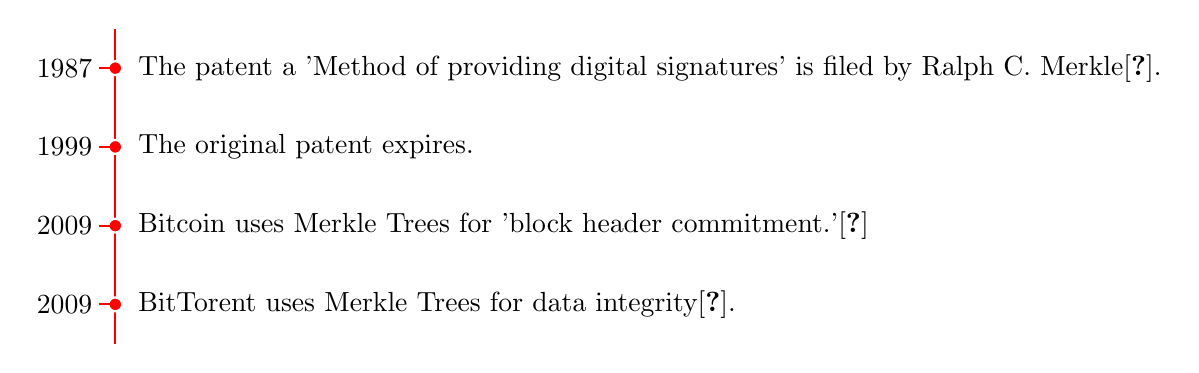
\begin{tikzpicture}[scale=0.5,every node/.style={outer sep=5pt}]
		%Notation: {year, the title of the event}
		%NOTE! Everyting is zero-based
		\def\ourInfo{{
				{"1987"," The patent a 'Method of providing digital signatures' is filed by Ralph C. Merkle\cite{merkle-patent}."},
				{"1999","The original patent expires."},
				{"2009","Bitcoin uses Merkle Trees for 'block header commitment.'\cite{friedenbach_alm_2017}"},			
				{"2009","BitTorent uses Merkle Trees for data integrity\cite{bep30}."},
		}}
		\pgfmathsetmacro{\length}{3}% Zero based.
		
		% Loop through the array containing all events.
		\foreach \i in {0, ..., \length}{
			\pgfmathsetmacro{\year}{\ourInfo[\i][0]}% Get the left cell (year)
			\pgfmathsetmacro{\eventName}{\ourInfo[\i][1]}% Get the right cell (event name)
			\draw[thick,red] (0,-2*\i-2)--(0,-2*\i);% Draw vertical line
			\ifnum \i=0 % Should be in red text
			\draw(0,-2*\i-1) node[black, right, align = left]{\eventName};% Display the event name
			\draw(0,-2*\i-1) node[black, left] {\year};
			\else % Should be in black text
			\draw(0,-2*\i-1) node[right, black]{\eventName};% Display the event name
			\draw(0,-2*\i-1) node[left] {\year};% Display the year
			\fi
		}
		% Draw the bullet with the dash
		\foreach \i in {0, ..., \length}{
			\filldraw[draw = white, fill = red,thick] (0,-2*\i-1) circle (5pt);
			\draw[thick,red] (-12pt,-2*\i-1)--(0,-2*\i-1);
		}
	\end{tikzpicture}
\end{figure}

As stated above, Merkle trees were created in 1987 by Ralph Merkle for digital signatures\cite{merkle-patent}. In the initial patent, the nodes were used for signing and verification:

\begin{quote}
	To sign a message $M_i$ the signer selects a previously unused node (i.e., node $i$) from the infinite tree. The message signing key at this node is then used to sign this message. The sequence of nodes from the root of the tree (i.e., node 1) to node $i$ is then used to verify that the message signature is correct and has not been tampered with.\cite{merkle-patent}
\end{quote}

Once the Merkle tree patent expired Merkle trees were implemented in various open-source projects including Bitcoin and BitTorrent which is expanded upon in a section below.

\section{Literature Review}

Merkle Trees are a component of several projects, as such many papers provide incremental changes towards certain operations on Merkle trees. This paper references the original patent by Ralph Merkle \cite{merkle-patent} in addition to descriptions of Merkle tree operations given by Boneh and Shoup \cite{boneh2020graduate}. As secondary sources, the implementation of Merkle trees in Bitcoin \cite{friedenbach_alm_2017} provides a real example of the impact of hash functions in addition to a whitepaper from the BitTorrent project\cite{bep30}.

\section{Construction}
 Merkle trees are constructed from the bottom up by hashing data as the leaf nodes.
 
 \begin{algorithm}[H]
 	\caption{Merkle tree construction}
 	\begin{algorithmic}
 		\For{$i = 1,\ldots, n$} \Comment{Compute leaf node hashes}
 		\State $y_i \leftarrow h(x_i)$  
 		\EndFor
 		 \For{$j= 1,\ldots, n-1$}  \Comment{Compute intermediate Nodes from $y_{n+1}, \ldots , y_{2n -1}$}
 		\State $y_{i+n} \leftarrow h(y_{2i-1}, y_{2i}) $ \Comment{Hash leaf nodes below for new hash}
 		\EndFor
 		\State \Return $Y$ \Comment{Return tree where $y_{2n-1}$ is the root}
 	\end{algorithmic}
 \end{algorithm}
 
When referring to the parts of a Merkle tree the most common terminology is "root hash" which refers to the hashed value of the root of the tree and "leaf hash" which refers to the hash for a given data block. 



\section{Operations}

There are several operations can for Merkle trees unrelated to tree manipulation that generate a proof resulting in a root hash. The root hash from the proof is then verified against a known hash to check for correctness. The most common operations are as follows.



\subsection{Proving Equality of Merkle Trees}

\begin{figure}[H]
	\begin{center}
		\begin{verbatim}
    ROOT1              ROOT2
   /     \             /     \
  L1       R1         L2      R2
 /  \    /  \        /  \    /  \     
L1.1  ....  R1.2    L2.1 ... R2.2
		\end{verbatim}
	\end{center}
\end{figure}

Proving the equality of two Merkle trees is an $O(1)$ operation. The operation compares the root nodes of the two trees. If the root nodes match, then the trees are equal. 


\subsection{Proving Membership}

\begin{figure}[H]
	\centering
	\includegraphics[width=.8\textwidth]{../Images/merkle-example.png}
	\caption{Show "\textit{Germany}" exist in the tree\cite{buchannen_2022}}
	% The reason we only need nodes 1, 34 and 567, is that we can regenerate Node 12 and Node 1234 from these values. Bitcoin, for example, uses this method in order to check the validity of a transaction within the block. We can then add our transactions into a Merkle Tree, and produce a root hash. Within the block we can then add the root hash of the previous block and the root hash of the next block, and thus interlock the blocks into a chain:	
\end{figure}

Using the figure above as an example, to prove  "\textit{Germany}" is a member of the tree the verifier hashes "\textit{Germany}" and hashes it with its sibling node to find the parent node. The parent node is then hashed with its sibling and the process repeats until the root node. The generated root node is compared with the known root node, should the hashes match then the element is verified. Proving membership requires checking $\log(n)$ tree levels, thus the operation takes $O(\log(n))$ time. 

Another advantage to checking membership using a Merkle tree is that checking the membership of multiple leaf nodes can be done in $O(\log(n))$. In the example above by proving "\emph{Germany}" was a member of the tree, the verifier also verified that "\emph{France}" was a member of the tree.

\subsection{Proving Non-Membership}

	\begin{figure}[H]
		\centering
	\includegraphics[width=.8\textwidth]{../Images/merkle-example.png}
	\caption{Show $x$ is not in the tree\cite{boneh2020graduate}}
	%possible.
\end{figure}

While hashing a value and checking if it appears in the leaf nodes might appear to Non membership cannot be verified using a standard Merkle tree. Non membership can only be proven with a sorted Merkle tree.  Dan Boneh and Victor Shoup provide the following  algorithm:
\begin{quote}
	To produce the proof, the prover first locates the two adjacent leaves $x_i$ and $x_{i+1 }$in T that bracket $x$, namely $x_i < x < x_{i+1}$. Next, the prover provides a Merkle proof that $x_i$
	is in position $i$ in $T$, and that $x_{i+1}$ is in position $i + 1$ in $T$. The verifier can check that these two leaves
	are adjacent, and that $x_i < x < x_{i+1}$, and this proves that $x$ is not in $T$. 
	\end{quote}
	
This operation takes $O(\log(n))$, but the additional requirement that the Merkle tree be sorted limits what operations can be used on the Merkle tree, notably merging.

\subsection{Merging Merkle Trees}

\begin{figure}[H]
    \begin{center}
	\begin{verbatim}
             ROOT
             /   \
           /       \
         /           \
       /               \
     ROOT1              ROOT2
   /     \             /     \
 L1       R1         L2      R2
 /  \    /  \       /  \    /  \     
L1.1  ....  R1.2   L2.1   ...   R2.2
\end{verbatim}
 \end{center}
\end{figure}


Merging Merkle trees is an $O(1)$ operation of the root of two other Merkle trees and creates a new root node. This operation can be used to add individual nodes to a Merkle tree, but it creates an unbalanced tree.



\section{Security}


\subsection{Authenticated Data Structure}

As defined by Boneh and Soup, Merkle Trees are secure data structures composed of three algorithms $D = (H, P, V )$\cite{boneh2020graduate}:
\begin{itemize}
	\item $H$ a secure hash function
	\item $P$ a proof function that takes an element, location, and structure $(i, x, T)$ and returns a proof of a given element
	\item $V$ a verification algorithm $V (i, x, y, \pi)$ that "accepts" or "rejects" a proof.
\end{itemize}

\subsection{Merkle Tree Attack Game}



The attack game for Merkle trees is defined in Boneh and Shoup using the definition of an authenticated data structure. Given a Merkle tree $D = (H, P, V )$ defined over $(\mathcal{X}^{n}, \mathcal{Y})$, and a given adversary $\mathcal{A}$: 

\begin{quote}
	The adversary $A$ outputs a $y \in \mathcal{Y}$, a position $i \in \{1, \ldots , n\}$, and two pairs $(x, \pi)$ and $(x', \pi')$ where $x, x' \in \mathcal{X}$.
\end{quote}

$\mathcal{A}$ wins the game if $x \neq x'$ and $V(i, x, y, \pi)=V(i, x', y, \pi')=$accept. Define $\mathcal{A}$'s advantage with respect to $\mathcal{D}$, denoted $\mathrm{ADSadv}[\mathcal{A}, \mathcal{D}]$, as the probability that $\mathcal{A}$ wins the game\cite{boneh2020graduate}.

\subsection{Security Proof}

Using the definition of the authenticated data structure combined with the attack game above, the security of the Merkle tree is dependent on the underlying hash function. 

The goal of the attacker is to generate a proof of membership at a given location. This can be reduced to creating a hash collision where the root node will be the same.

In the case of a Merkle tree with only one leaf node, the attacker would need to generate a collision $c$ such that if $H(x) = x'$, then $H(c)=x'$ but $x\neq c$.

In the case of a Merkle tree with two leaf nodes, the attacker can create a collision by colliding on the hash of the leaf node or by colliding against the root node. Let $a, b$ be the data blocks and let $H(a)=a', H(b)=b'$ which gives a root node $H(a'b')=r$. The attacker can either find $H(c)=c'$ such that $c' = a'$, $c'=b'$ or $H(c'b') = r$, $H(a'c') = r$. All attacks depend on a flaw in the hash function.

More generally, $x \in T$ with hash $H(x) = h$ at position $i$. Let the attacker create a collision such that $H(y) = h$ but $x \neq y$. Thus the attacker's advantage against a Merkle tree is the same as the attacker's advantage against the hash function used by the Merkle tree.


\section{Use Cases}

Merkle trees are used as authenticated data structures with optimal complexity for proving membership and comparing against other structures. 

\subsection{Bitcoin} \label{sec:Bitcoin}

Bitcoin, and other cryptocurrencies, use Merkle trees for the commitment header.  The \textit{chain} in blockchain refers to the chain of receipts from processed transactions. It would be too slow to create a receipt for each transaction, so Bitcoin groups transactions into sections. The smaller group of transactions is a Merkle tree where the leaf nodes represent a single transaction. Thus the group of transactions results in a root hash which is used as the commitment header.

Merkle trees were incorrectly implemented in the Bitcoin protocol. This implementation resulted in DOS attacks due to over-hashing and duplicate nodes (CVE-2012-2459). This bug was patched in a proposal that replaced the Merkle tree implementation\cite{friedenbach_alm_2017}.


\subsection{BitTorrent Data Integrity} \label{sec:BitTorrent}

BitTorrent uses Merkle trees for checking the integrity of torrented files. The torrented data is hashed into a Merkle Tree and the root hash is compared with a trusted peer to verify integrity\cite{bep30}. If the root hashes do not match then the nodes below are compared with the trusted peer. This process repeats until a non-matching block is reached. The advantage of using a Merkle tree over another data structure is finding corrupted data blocks in $O(\log(n))$ time. 

\section{Closing}

Merkle trees were not the first authenticated data structure, the Merkle Damgard construction provides several of the same operations \cite{boneh2020graduate}, but the number of properties in Merkle trees makes them desirable across a multitude of applications. The core construct of Merkle Trees, the tree, enables $O(\log (n))$  time operations in addition to speed-ups for proofs of many members. Their usage in various applications, notably in most cryptocurrencies, serves as evidence that Merkle trees will continue to propagate. 



\newpage

\printbibliography


\end{document}
